
\setcounter{chapter}{2}
\chapter{Sprint 1: Project Launch}
\minitoc %insert la minitoc
\graphicspath{{Chapter3/figures/}}

%\DoPToC
%==============================================================================
\pagestyle{fancy}
\fancyhf{}
\fancyhead[R]{\bfseries\rightmark}
\fancyfoot[R]{\thepage}
\renewcommand{\headrulewidth}{0.5pt}
\renewcommand{\footrulewidth}{0pt}
\renewcommand{\chaptermark}[1]{\markboth{\MakeUppercase{\chaptername~\thechapter. #1 }}{}}
\renewcommand{\sectionmark}[1]{\markright{\thechapter.\thesection~ #1}}

\begin{spacing}{1.2}

%==============================================================================

\section*{Introduction}
This chapter is introducing the software development disciplines and rules followed during the achievement of our project. In order to have a clear development structure, a development process must be set in place in the earliest stage of our project life.

Our development process is a combination of different practices like Test-driven development and DevOps.

\section{Kanban Tickets Life Cycle}
Following the Kanban methodology our project is decomposed to small tickets with limited scopes. The tickets are developed in an incremental way following a priority order, and together they shape our project to it's final version.
\begin{figure}[H]\centering
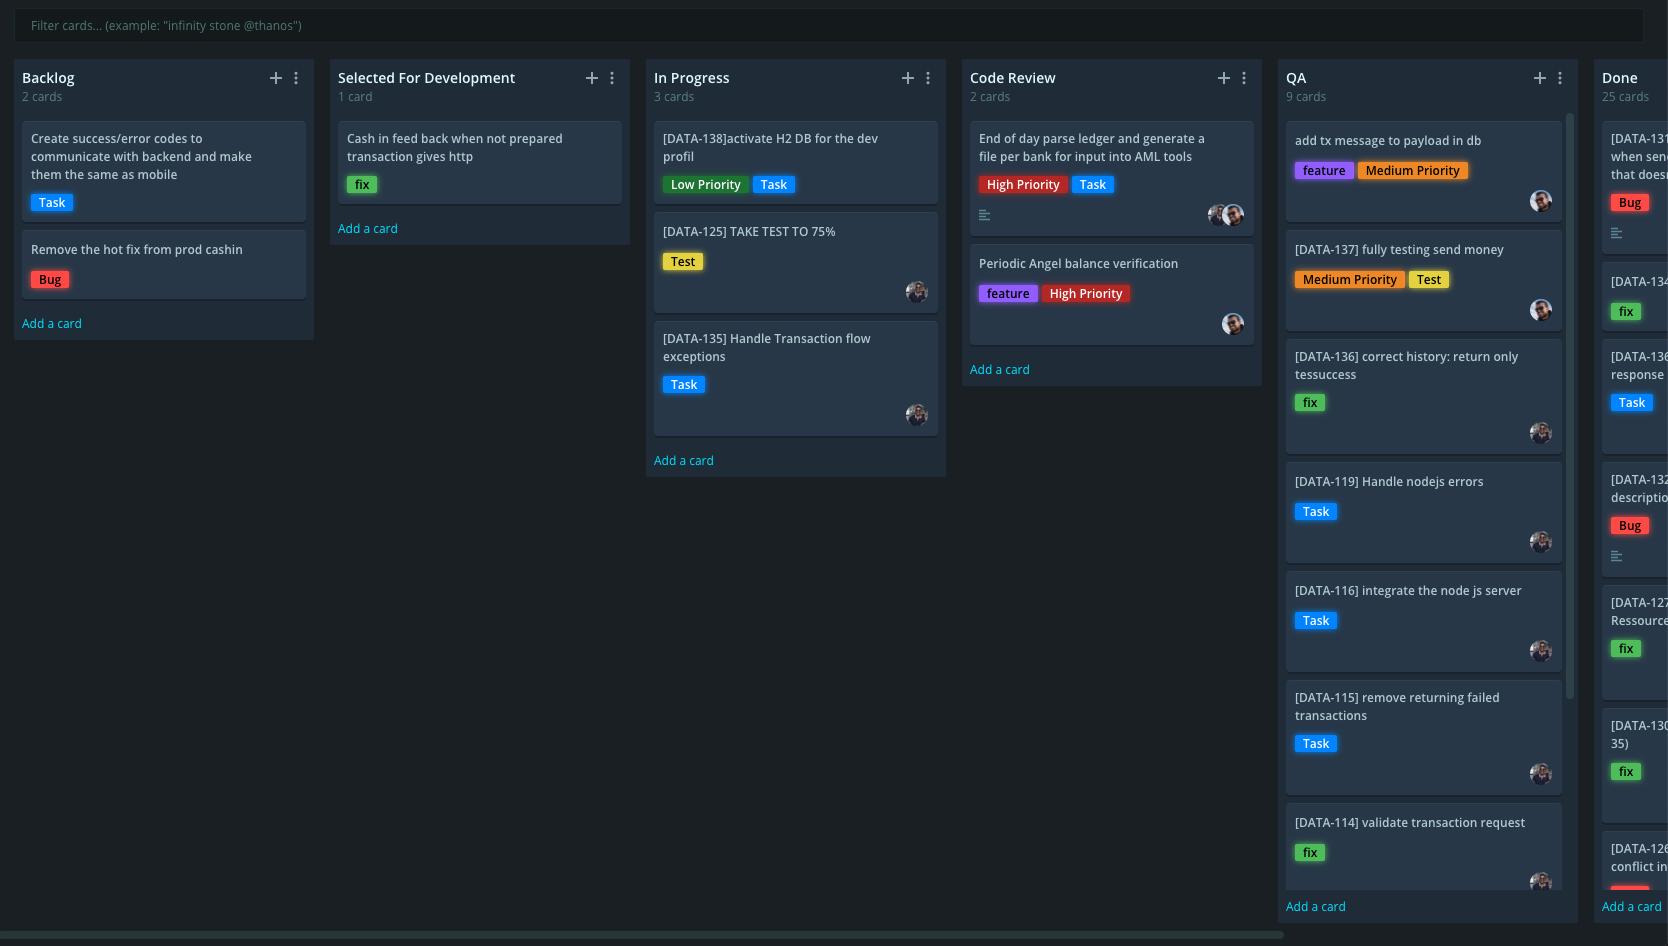
\includegraphics[scale=0.3]{kanban_board.png}
\caption{Kanban Board}
\label{fig:fig1}
\end{figure}
\subsection{Backlog}
All tickets are created in the "Backlog" stage, any work that needs to be done is formed into a ticket.


The ticket needs to have a self-explanatory description, to make it simple for the developer to start working on it without the need for further explanation.

A Tag must be assigned to the ticket as well, tags could be referring to the nature of the work to do (Bug, Fix, Task\dots), or the scope (Back-end, Front-end, DevOps\dots).

In the end the ticket priority must be set following a priority system set by the development team. The system could relay on numerical values (0 having the least priority, 1, 2 \dots), or having specific tags (LOW, MEDIUM, HIGHT, URGENT) which we will be using in our project.

Tickets could only move from "Backlog" to "Selected For Development".
\subsection{Selected For Development}
In the "Selected For Development" stage developers have access to the tickets. They have to tackle the ticket following the priority system and the tag matching their expertise (Back-end, Front-end).

Once they choose a ticket they must assign it to their name, move it to the "In Progress" stage and create a git branch with the ticket name and finally start developing.

Tickets could only move from "Selected For Development" to "In Progress".
\subsection{In Progress}
The "In Progress" stage serve as safety mechanism to avoid having two developers working on the same ticket.

This stage indicates that the tickets is being taking care of, it also shows the person developing the ticket.

If the developer finish his work he should move the ticket to "Code Review" stage and make a pull request of the branch.


In the case of failure ticket should go back to "Selected For Development" stage.
\subsection{Code Review}
Once a ticket is in the "Code Review" stage, the project manager should open the pull request and check the code committed by the developer.

In case of approval the pull request is merged and deployed, the ticket then is moved to "QA".


In case of disapproval the project manager leaves comments on the pull request and moves the ticket back to "In progress". The developer then needs to check the code and fix the issue.
\subsection{QA}
In the "QA" stage tickets are tested by fellow developers, the functionality of the ticket should be tested on an environment similar to the production environment, also developer should push the test to the limit and test all edge cases.

If all developers approve that the code is working fine in every possible scenario the ticket is moved to done, otherwise the ticket info should be updated with the issues encountered and the ticket is moved back to the "In Progress" stage.

\subsection{Done}
All tickets should finally be moved to the "Done" stage, this stage groups all the work done and keeps track of the progress of the development.


After a fixed time tickets get archived to gain space in the Kanban board.
\section{Gitflow workflow }
\begin{figure}[!ht]\centering
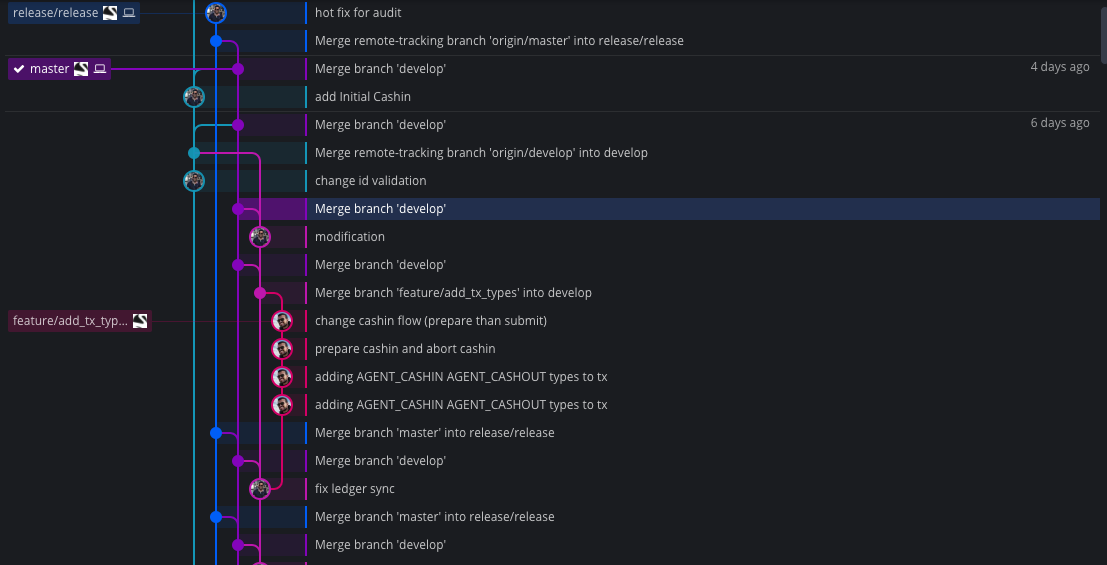
\includegraphics[scale=0.4]{git_workflow.png}
\caption{Git Workflow}
\label{fig:fig1}
\end{figure}
Gitflow Workflow is a Git workflow design that was first published and made popular by Vincent Driessen at nvie. The Gitflow Workflow defines a strict branching model designed around the project release. This provides a robust framework for managing larger projects.

Gitflow is really just an abstract idea of a Git workflow. This means it dictates what kind of branches to set up and how to merge them together.
\subsection{Feature Branch}
The feature branch is created by the developer for every Kanban ticket he tackles. When moving the ticket to the "In Progress" stage the branch should be created with the same name as the ticket.

All the development specific to the scope of the ticket should be done in the same branch, and in the end the developer should make a pull request on the Develop Branch.
\subsection{Develop Branch}
The Develop branch present the edge version of the product, it contains all new developed features. This branch is the main branch to the internal project team, All newly developed feature are tested by developers on this branch, it maps to the "dev environment".

This branch could present a number of bugs because by nature it's a testing and validation branch of the latest developed code.

This branch is daily updated.
\subsection{Master Branch}
After tickets validation and bug fixes, the internal team merge a stable version of the product (Develop branch) to the Master branch. This branch maps to the staging environment and serves for testing on the company level.

All company projects depending on our project always use its staging version. The testing and integration with other projects should be verified extensively before merging to the production environment.


\subsection{Release Branch}
This is the production branch, code on this branch has been tested twice in both the dev and staging environments.

The branch is updated according to the release dates, it's the result of merging a stable master branch.

The branch maps to the prod environment and it's the actual branch used by the end user.
\subsection{Hotfix Branch}
As it is impossible to have a bug free software, we should take in consideration bugs popping in the prod environment.

Every bug discovered on the prod environment opens an urgent fix ticket, the ticket branch is based on the release branch and its merged directly to the release branch after the fix.

This is a measure to quickly fix issues that have effects on the end user.
\section{Test-driven development}
Test Driven Development is a development technique that requires the writing of tests even before writing the first line of code.

In theory, the method requires the intervention of at least two different people, one person writes the tests, the other writes the code. This avoids problems related to subjectivity.

In practice things are more complicated, sometimes you develop alone or you write the tests yourself that guarantee the integrity of a new functionality in a collaborative project.

The TDD can be divided into 5 distinct steps:
\begin{enumerate}
	\item  Write a test.
	\item Check that it fails.
	\item Write the code enough for the test to pass.
	\item Check that the test passes.
	\item Optimize the code and check that there is no regression.
\end{enumerate}

\begin{figure}[!ht]\centering
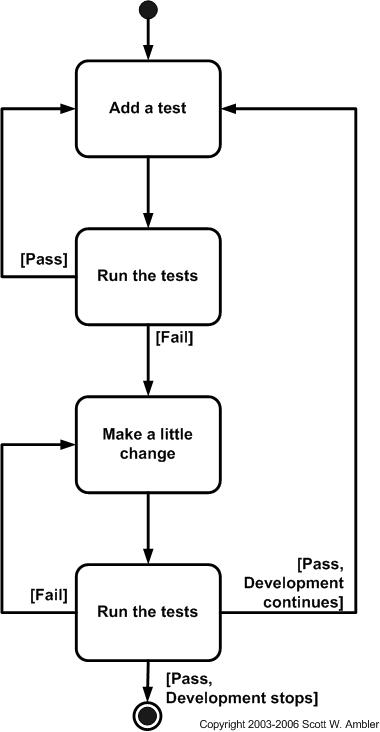
\includegraphics[scale=0.6]{tddSteps.jpg}
\caption{TDD Steps}
\label{fig:fig1}
\end{figure}
\newpage
In our project, The development of every ticket starts by writing the test. A pull request can only be approved if it contains and passes the new test.

This discipline enable our project to benefits from the DevOps world, As it's important to have test for the CI-CD process to be defined.


\section{DevOps}
DevOps is a set of practices that automates the processes between software development and IT teams, in order that they can build, test, and release software faster and more reliably.

In our project we need to have an autonomous testing and deployment process to maintain our three environments:
\begin{itemize}
	\item \textbf{Dev environment:} Represents the Develop branch and used for internal team testing.
	\item \textbf{Staging environment:} Represents the Master branch and used for a company level testing.
    \item \textbf{Prod environment:} Represents the Release branch and used by the end user.
\end{itemize}

\subsection{DevOps Steps}
With every branch push our CI-CD server (Jenkins) triggers an automatic script that consists of a set of predefined steps.

The steps behave slightly different according to the branch name.
\begin{figure}[!h]\centering
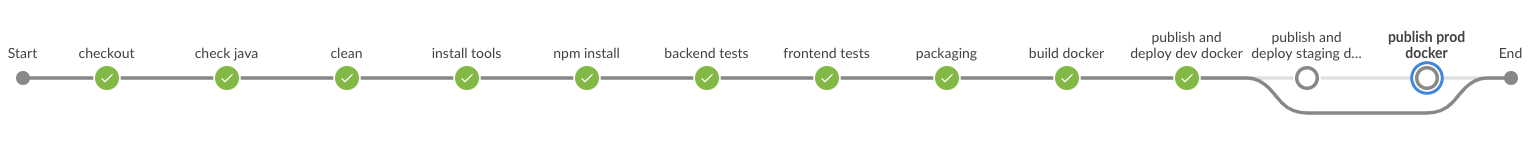
\includegraphics[scale=0.3]{jenkins.png}
\caption{Kaoun logo�}
\label{fig:fig1}
\end{figure}
\subsubsection{Preparation}
The first step of every build is getting the branch code and preparing a clean environment containing all the dependencies required to run our project.
\subsubsection{Testing}
In this step all tests are executed for both backend and frontend. A full report is created with the test results.
We can only continue the build if all tests are passed gracefully otherwise the job is terminated.
\subsubsection{Quality Measurements}
In this steps the code is inspected by the open-source platform SonarQube.

The step performs automatic reviews with static analysis of code to detect bugs, code smells, and security vulnerabilities.
\subsubsection{Dockerization}
If all testing and quality measures are approved we proceed to the Dockerization of our project.
This step creates a standard artifact that can be deployed on any infrastructure without the need of specific configurations for different servers.

If the Docker images is created successfully, it will be tagged latest and pushed to the Docker Hub.

\subsubsection{Deployment}
In the last step of the build, and according to the branch name the new artifact is deployed to the convenient server (dev, staging, prod).

On every target server we have a docker swarm cluster to deploy the new version of the product.
The swarm cluster is also configured with the different environment variables as secrets to protect the different credentials (database, cloud services\dots).
\section{Tools}
In the section we will present the set of tools that make it possible to follow the development disciplines mentioned above. The tools also help the automation of the processes.
\subsection{Adobe XD}
Adobe XD is a vector-based tool developed and published by Adobe Inc for designing and prototyping user experience for web and mobile apps.
\subsection{Bitbucket}
Bitbucket is a web-based version control repository hosting service owned by Atlassian, for source code and development projects that use Git revision control systems.
\subsection{GitKraken Glo Boards}
GitKraken Glo Boards is a software that manage boards and tickets. In our case the Kanban board is created and managed on GitKraken.
\subsection{Docker}
Docker is a tool designed to make it easier to create, deploy, and run applications by using containers. Containers allow a developer to package up an application with all of the parts it needs, such as libraries and other dependencies, and ship it all out as one package. By doing so, thanks to the container, the developer can rest assured that the application will run on any other machine regardless of any customized settings that machine might have that could differ from the machine used for writing and testing the code.
\subsection{Docker Swarm}
As a platform, Docker has revolutionized the manner software was packaged. Docker Swarm or simply Swarm is an open-source container orchestration platform and is the native clustering engine for and by Docker. Any software, services, or tools that run with Docker containers run equally well in Swarm. Also, Swarm utilizes the same command line from Docker.

Swarm turns a pool of Docker hosts into a virtual, single host. Swarm is especially useful for people who are trying to get comfortable with an orchestrated environment or who need to adhere to a simple deployment technique but also have more just one cloud environment or one particular platform to run this on.
\subsection{Jenkins}
In order to have our CI/CD environment, we used Jenkins which is an open source automation server that helps you to automate the non-human part of the software development process.

Jenkins is a stand-alone open source automation server that can be used to automate all kinds of tasks related to software creation, testing, delivery or deployment.
\subsection{SonarQube}
SonarQube (formerly Sonar) is an open-source platform developed by SonarSource for continuous inspection of code quality to perform automatic reviews with static analysis of code to detect bugs, code smells, and security vulnerabilities on 20+ programming languages.

SonarQube offers reports on duplicated code, coding standards, unit tests, code coverage, code complexity, comments, bugs, and security vulnerabilities.

\section*{Conclusion}
In this chapter we set the development disciplines to follow in the making of our project.

We went through the Kanban methodology in practice, explaining the different steps of the incremental code writing.

 We also set the rules of the git branching model we will be using in our development process, as well as  the test-driven development discipline to follow for every branch.

We tackled our DevOps setup and the different steps of the automation process from code writing to project deployment.

In the end we presented the tools we will be using in our project development life cycle.


%==============================================================================
\end{spacing}
